\chapter{Conceitos Básicos}

\section{Grafos}
Muitas situações no mundo real podem ser descritas com o uso de um diagrama, composto este por conjunto de pontos e arestas, onde as arestas unem pares desses pontos. Por exemplo, os pontos podem representar cidades em um mapa, e as arestas representariam as estradas que ligam duas cidades. O conceito de grafo parte de uma abstração matemática para caracterizar situações com essas características (\cite{Bondy1976}).

Um grafo $G$ é uma tripla ($V$, $E$, $\psi$), consistido por um conjunto não vazio de vértices $V$, um conjunto de arestas $E$ e uma função de incidência $\psi$ que caracteriza quais vértices possuem uma relação (através de uma aresta) com outros vértices. Por exemplo, seja $G = (V, E, \psi)$ um grafo (figura \ref{fig:graphExample1}), tal que $V = \{0, 1, 2, 3, 4, 5\}$, $E = \{a, b, c, d, e, f, g, i\}$ e $\psi$ a função incidência representada na tabela \ref{tab:graphExample1}.

\begin{table}[ht!]
\caption{Função incidência $\psi$ de $G$}
\label{tab:graphExample1}
\centering
\begin{tabular}{| c | c |}
\hline
    $\psi_a = 1,2$\\ 
    $\psi_b = 2,0$\\ 
    $\psi_c = 1,0$\\ 
    $\psi_d = 4,3$\\
    $\psi_e = 4,5$\\
    $\psi_f = 5,3$\\
    $\psi_g = 2,5$\\
    $\psi_h = 1,4$\\
    $\psi_i = 4,3$\\
\hline
\end{tabular}
{\fontsize{11pt}{\baselineskip}\selectfont
\\Fonte: Elaborado pelo autor.
}
\end{table}

Segundo \cite{Bondy1976}, grafos possuem este nome porque eles possuem uma representação gráfica, e são essas representações que facilitam o entendimento de suas propriedades.

\begin{figure}[ht!]
\caption{Diagrama do Grafo $G$}
\label{fig:graphExample1}
\centering
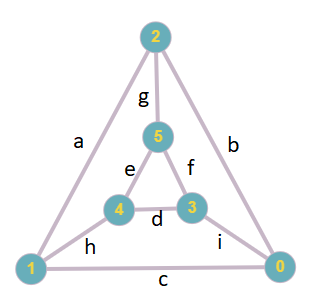
\includegraphics[scale=0.75]{img/graphExample1.png}
{\fontsize{11pt}{\baselineskip}\selectfont
\\Fonte: Graph Online\footnotemark
}
\end{figure}
\footnotetext{Disponível em: \url{https://graphonline.ru/en/}}

\section{Redes Neurais Artificiais} %aqui falarei sobre redes neurais, somente introduzi grafos para pode explicar por completo ela
O ser humano possui capacidades cognitivas extraordinárias e, desde o surgimento da computação, desejou-se projetar máquinas capazes de realizar tarefas inteligentes que, até então, somente eram  executadas por humanos. O primeiro trabalho desenvolvido nessa área foi apresentado por (\cite{mcculloch1943logical}) que, por sua vez, também foi utilizado como base para a concepção do \textit{Perceptron} (\cite{rosenblatt1958perceptron}) e um modelo semelhante, o \textit{Adaline} (\cite{widrow1960adaptive}). Tais trabalhos deram origem ao conceito de Redes Neurais Artificiais (RNA) que, em outras palavras, é uma tentativa de copiar a estrutura e o funcionamento do cérebro, composto este por bilhões de neurônios, para uma estrutura artificial, transformando assim as redes neurais biológicas em redes neurais artificiais (\cite{Rauber2005}).

Para compreender o conceito por trás de uma rede neural, é preciso introduzir um modelo simplificado de um neurônio e suas capacidades de processamento associadas. Cada neurônio é considerado como uma unidade básica de processamento que, quando estimulada por sinais de entrada, emitem sinais de saída como uma reação. Tais sinais emitidos por um neurônio, são repassados para outros neurônios através de uma conexão sináptica. Tal processo pode ser repetido por várias camadas de neurônios até chegar ao nosso cérebro, que então processa essa informação e produz novas reações. (\cite{baeza1999modern}). A principal função de uma rede neural é armazenar conhecimento experimental e torná-lo disponível, o que em prática significa que este conhecimento é adquirido e armazenado em pesos sinápticos durante o processo.

Uma RNA é normalmente implementada através de um programa de computador (\textit{software}) ou através de componentes eletrônicos (\textit{hardware}). Uma rede neural pode ser representada matematicamente através de uma estrutura de grafo (figura \ref{fig:graphNeuron}), onde os vértices fazem o papel dos neurônios e as arestas representam as conexões sinápticas entre os neurônios, onde se adicionarmos pesos a tais arestas, é possível mensurar a "força" de tal conexão sináptica. Seja $x_i$ entradas fornecidas por outros neurônios para um neurônio artificial. O processamento desse neurônio consiste em uma combinação linear das $D$ entradas tais que $\sum_{i=1}^{D} = w_i x_i$, onde $x_i$ é uma aresta com peso $w_i$. Se tal valor ultrapassar um limiar $\mu$, esse neurônio dispara um valor positivo (1) na saída binária $y$, caso contrário dispara um valor negativo (0) na saída. 

\begin{figure}[ht!]
\caption{Diagrama de um neurônio artificial}
\label{fig:graphNeuron}
\centering
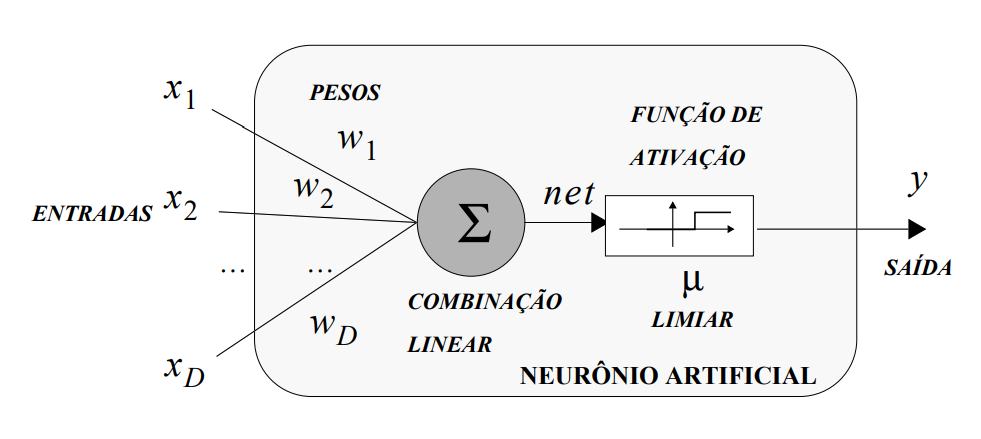
\includegraphics[scale=0.5]{img/graphNeuron.png}
{\fontsize{11pt}{\baselineskip}\selectfont
\\Fonte: RAUBER, 2005. p 6.
}
\end{figure}